\begin{figure}[htbp]
\centering
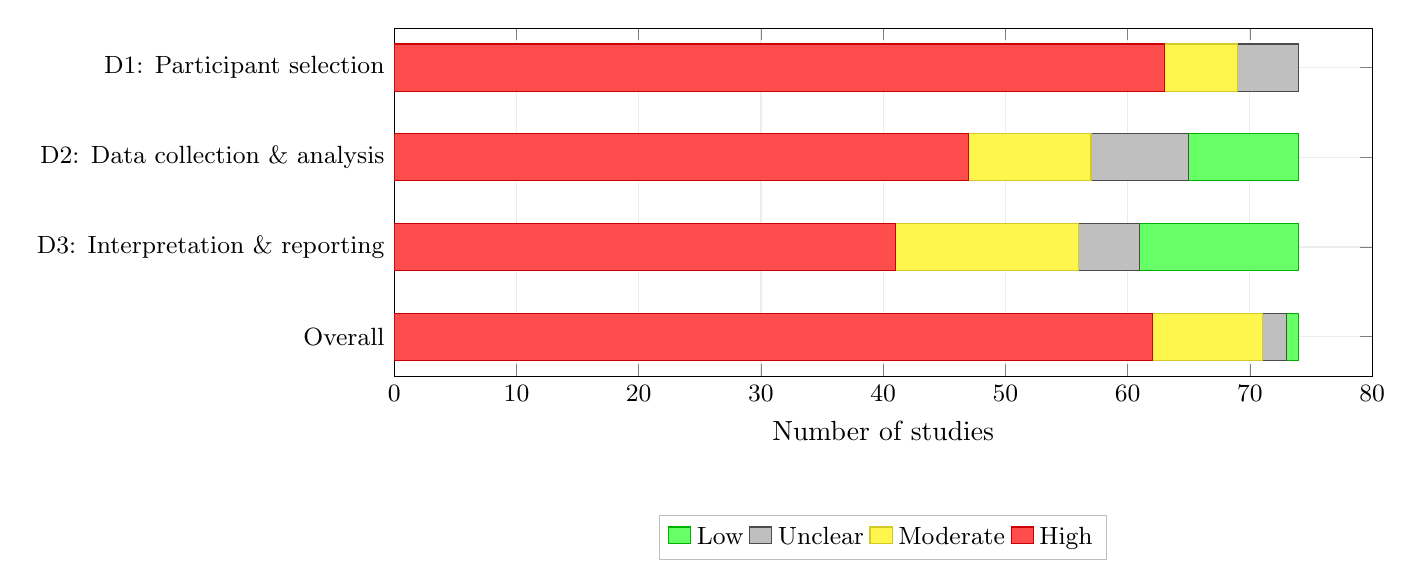
\begin{tikzpicture}
\begin{axis}[
    xbar stacked,
    width=14cm,
    height=6cm,
    xlabel={Number of studies},
    xmin=0, xmax=80,
    ytick=data,
    yticklabels={
        {Overall},
        {D3: Interpretation \& reporting},
        {D2: Data collection \& analysis},
        {D1: Participant selection}
    },
    yticklabel style={font=\small},
    xticklabel style={font=\small},
    legend style={at={(0.5,-0.40)}, anchor=north, legend columns=4,
        font=\small, draw=gray!50},
    bar width=0.6cm,
    enlarge y limits={abs=0.5cm},
    grid=major,
    grid style={gray!15, thin},
    xtick={0,10,20,30,40,50,60,70,80},
    reverse legend,
]
\addplot[fill=red!70, draw=red!80!black] coordinates {
    (62, 0) (41, 1) (47, 2) (63, 3)
};
\addplot[fill=yellow!70, draw=yellow!80!black] coordinates {
    (9, 0) (15, 1) (10, 2) (6, 3)
};
\addplot[fill=gray!50, draw=gray!60!black] coordinates {
    (2, 0) (5, 1) (8, 2) (5, 3)
};
\addplot[fill=green!60, draw=green!70!black] coordinates {
    (1, 0) (13, 1) (9, 2) (0, 3)
};
\legend{High, Moderate, Unclear, Low}
% Percentage labels on high-risk bars
\node[font=\scriptsize, text=white, anchor=east] at (axis cs:60, 0) {83.8\%};
\node[font=\scriptsize, text=white, anchor=east] at (axis cs:39, 1) {55.4\%};
\node[font=\scriptsize, text=white, anchor=east] at (axis cs:45, 2) {63.5\%};
\node[font=\scriptsize, text=white, anchor=east] at (axis cs:61, 3) {85.1\%};
\end{axis}
\end{tikzpicture}
\caption{Risk-of-bias ratings by domain and overall ($n = 74$). The gradient from Domain~1 (85.1\% high) to Domain~3 (55.4\% high) indicates that participant selection is the most persistent source of weakness, while interpretive practices are relatively stronger.}
\label{fig:rob-domains}
\end{figure}
